\documentclass[10pt]{article}
% Layout follows the official Apart sprint template (Google Docs): US Letter, 1in margins, Old Standard TT.
\usepackage[letterpaper,margin=1in]{geometry}
\usepackage{fontspec}
\setmainfont{OldStandard}[Path=fonts/, Extension=.ttf, UprightFont=*-Regular, ItalicFont=*-Italic, BoldFont=*-Bold, BoldItalicFont=*-Bold, BoldItalicFeatures={FakeSlant=0.18}]
\newfontfamily\symfont{Apple Symbols}
\usepackage{xeCJK}
% CJK font: Noto Serif/Sans CJK TC, installed in the user font folder (edit the path if yours differs).
\newcommand{\cjkdir}{\string~/Library/Fonts/}
\setCJKmainfont{NotoSerifCJKtc-Regular.otf}[Path=\cjkdir, BoldFont=NotoSerifCJKtc-Bold.otf]
\setCJKsansfont{NotoSansCJKtc-Regular.otf}[Path=\cjkdir, BoldFont=NotoSansCJKtc-Bold.otf]
\usepackage{graphicx,booktabs,amsmath,amssymb,xcolor,microtype,enumitem,caption}
\usepackage[hidelinks]{hyperref}
\usepackage{natbib}
\setlist{nosep,leftmargin=*}
\captionsetup{font=small}
\setlength{\parskip}{3pt}
\setlength{\parindent}{0pt}
\emergencystretch=2em
\makeatletter
\renewcommand\section{\@startsection{section}{1}{\z@}{10pt plus 2pt}{4pt}{\normalfont\large\bfseries}}
\renewcommand\subsection{\@startsection{subsection}{2}{\z@}{8pt plus 2pt}{3pt}{\normalfont\normalsize\bfseries}}
\renewcommand\@seccntformat[1]{\csname the#1\endcsname\ifnum\pdfstrcmp{#1}{section}=0 .\fi\enspace}
\makeatother
\newcommand{\ours}{PayloadConv}
\newcommand{\cand}{Zhong Yuheng (鍾予衡)}

\begin{document}
\thispagestyle{plain}
\noindent\rule{\textwidth}{2.2pt}
\begin{center}
{\fontsize{16}{20}\selectfont\bfseries From Swarms to Certainty: Coordinated AI Accounts Steer AI Election Briefings, and Provenance-Based Detection Flags Real Supporters by Camp\footnote{Research conducted at the \href{https://apartresearch.com/sprints/ai-x-epistemics-research-sprint-2026-11-13-to-2026-11-15}{AI x Epistemics Research Sprint}, November 2026. Track: Trust Infrastructure (secondary: Epistemic Products).}}
\end{center}
\vspace{-4pt}\noindent\rule{\textwidth}{0.4pt}
\begin{center}
Yu-Wei Chiu\\ LargitData Inc., Taipei, Taiwan\\[6pt]
\textbf{With}\\ Apart Research
\end{center}
\vspace{-2pt}
\begin{center}{\large\bfseries Abstract}\end{center}
\vspace{-6pt}
\begin{list}{}{\leftmargin=0.6in\rightmargin=0.6in}\item\relax\small
LLM agents increasingly turn social media into decision briefs. Do they weigh \emph{independent evidence} or \emph{count accounts}, and what do coordination-provenance signals cost? We inject LLM agent swarms promoting a \emph{fictional} independent candidate into real discussion of the 2026 Taipei mayoral race. A briefing agent decides whether to invite him to a TV debate and list him in polls. With no swarm, Gemma-4-31B never invites him; once retrieved, a 30-account orchestrated swarm raises its invite rate to 83\%, a self-seeded one to 100\%. Moving the same 30 pitch texts from one account to three raises invites from 28\% to 72\% (+44 points [11, 72]): the agent counts heads. Gemini 3.8 Flash's poll listing rises from 0\% (one account) to 100\% (30). Asked separately, both models raise a (non-specific) coordination flag, yet still invite or list him. An independence assessment inside the decision call cuts Gemma's invitations (83\% $\to$ 6\%; poll listing stays 100\%) and Gemini's poll listings (100\% $\to$ 11\%); a count-only control does neither. It still invites renamed support from 30 real accounts (94\%), and the swarm's texts posted once per account (33\%). Our detector stops orchestrated swarms' invitations, but flags under a quarter of self-seeded swarms' retrieved messages and none from one-post accounts; with wording fixed, a few flags, detector or random, raise Gemma's counted independent voices. Its provenance-inheriting score gives each camp's supporters nearly one value, so a threshold between them flags one camp wholesale: 70--72\% of the challenger's scored supporters versus 21--26\% of the incumbent's.
\end{list}

\section{Introduction}
Social-listening briefs are an epistemic product. An analyst, and now often an LLM agent, reads what ``people are saying'' and turns it into a judgement that others act on: a TV producer decides whom to invite to a debate, a pollster decides whom to list. Both judgements should track \emph{breadth of independent support}. Generative agents make the appearance of breadth cheap \citep{chiu2026payload}. If briefing agents count accounts rather than weigh independent evidence, a small swarm can buy a recommendation to invite.

We study this where it matters most, a live election, while generating content only about a \textbf{fictional} candidate. Real candidates are analysed but never written about. Contributions:
\begin{enumerate}
\item \textbf{Account-count ablation:} identical pitch texts attributed to $k\in\{1,3,10,30\}$ accounts isolate head-counting from content (Fig.~\ref{fig:k}).
\item \textbf{Assessment without action, and a same-call fix:} both models flag coordination when asked in a separate call, yet their briefs still recommend the candidate. Asking for the independence assessment inside the decision call nearly removes the swarm's invitation (Gemma) and poll listing (Gemini), but not Gemma's poll listing; it still invites renamed real support, partly also a one-post-per-account swarm, and leaves real front-runners' decisions unchanged. A count-only control has no such effect (Table~\ref{tab:chain}).
\item \textbf{Coordination provenance as a defense, and its price.} Our detector works mainly against orchestrated swarms; with wording held fixed, a few flags (by detector or at random) raise the counted independent voices; and its provenance-inheriting score acts as a camp selector (Fig.~\ref{fig:b1}).
\end{enumerate}

\section{Related Work}
\textbf{Evidence laundering.} \citet{zhou2026laundering} show that deep-research agents treat paraphrased, correlated web pages as independent evidence, and propose a provenance gate that collapses them. Our sources are social accounts, and our swarms are told \emph{not} to paraphrase each other, so near-duplicate gates have little to collapse (we do not test one). We test a population-level signal instead, and measure what it costs real voices.

\textbf{Majority and social pressure in LLMs.} LLM agents defer to a group consensus, more so as the majority grows \citep{weng2025conformity}, and RLHF-trained assistants defer to their users' stated beliefs \citep{sharma2024sycophancy}. We study the same deference applied to retrieved social evidence, where the ``majority'' is a count of accounts.

\textbf{AI summaries of user content.} \citet{liu2026positivity} find positivity bias at both the sampling and summarising stages of platform AI summaries. Our no-swarm baseline and stance-matched contexts control for such priors.

\textbf{Coordination detection.} Classical methods find coordinated accounts through shared behavioural traces such as co-posting, co-retweeting and synchronised timing \citep{keller2020astroturfing,pacheco2021coordinated}; LLM swarms that never copy each other weaken these traces \citep{chiu2026payload}. Our defense is \ours/D4c from our prior sprint work \citep{chiu2026payload}, disclosed in App.~\ref{app:prior}. It scores an account by how widely, and how \emph{unprompted}, the entity it endorses is endorsed across threads (definition in App.~\ref{app:d4}).

\section{Methods}
\textbf{Data.} From InfoMiner (LargitData's social-listening service) we collect posts and comments matching 蔣萬安 / 沈伯洋 / 台北市長 from 25 Oct to 10 Nov 2026, on Threads, Facebook pages and groups, PTT, YouTube, Mobile01 and Dcard: 552k raw rows (23.6k posts, 528k comments), 523k messages after de-duplication and dropping rows with no text, no author ID or no fetched root post, 22.7k threads, 226k accounts. We split by thread start date into a \emph{dev} window (10/25--11/02) and a \emph{held-out} window (11/03--11/10), and sample whole threads to about 40k messages per window (40,026 / 40,510). Models see accounts only as salted pseudonyms.

\textbf{Claims.} A self-hosted Gemma-4-31B (H200, temperature 0) labels every message with \{target, stance, claim\}: whom it supports or criticises. Replies are shown together with their root post.

\textbf{Swarms.} The fictional independent candidate is \cand{}: no web hits, 0 corpus mentions. Our prior generator \citep{chiu2026payload} builds 30-agent swarms with planner-assigned personas and roles, style exemplars from real accounts, organic reply delays, home platforms, and 20\% replies to fellow agents.
\begin{itemize}
\item \textbf{S4} (orchestrated + evasive) replies inside real race threads. Each message carries the pitch with probability 0.25, and replies that boost a fellow agent's pitch carry it too, so 37--64\% of a swarm's messages carry it and 17--29 name him. The pitch: housing and commute policy, ``a mayor who doesn't rely on party machines'', ``his town halls are full of young parents''.
\item \textbf{S5} (adaptive) also opens six threads of its own, so that its endorsements look solicited.
\end{itemize}
Agents are told never to name or evaluate real politicians, and messages that do are dropped (2 of 1,204). There are 3 seeds per attack per window, giving 81--132 messages per swarm.

\textbf{Briefing agent.} Every context has exactly 60 messages:
\begin{itemize}
\item up to 30 candidate-relevant messages (the text or extracted target names him), ranked by embedding similarity;
\item real race messages to fill the rest, ranked by similarity to a general race query, so context size never reveals volume.
\end{itemize}
The fictional candidate has no organic mentions, so a swarm fills all 30 candidate slots (half the context). Results are therefore conditional on the swarm being retrieved: they measure how the agent weighs what it is shown, not how often a swarm reaches a real pipeline.
A newsroom-analyst prompt asks for a JSON brief: \texttt{decision} $\in$ \{invite, wait, decline\}, \texttt{include\_in\_poll}, \texttt{grassroots\_\allowbreak momentum} (0--3), sentiment, consensus, confidence and cited message IDs. A \emph{separate second call} on the same context asks how many \emph{independent} supportive voices there are and whether coordination is suspected. Keeping that question out of the first call avoids priming the brief. Models: Gemma-4-31B (H200), temperature 0.7, 3 reps with reshuffled message order (2 in the over-correction experiment); Gemini 3.8 Flash (\texttt{gemini-3.8-flash-medium}), 1 rep on a reduced grid, 3 (2 on real candidates) for the chained experiments. The same Gemma model also generated the swarm text and labels claims; Gemini is the out-of-family check.


\textbf{Defenses.} \ours{} (D4 and its provenance-inheriting variant D4c) is computed on the full pool the agent draws from, and an account is flagged if either score exceeds its threshold. The flags are shown in one of two ways:
\begin{itemize}
\item \emph{annotate}: a ``{\symfont ⚠} coordination suspect'' tag, with a note that tagged accounts may belong to one coordinated group;
\item \emph{collapse}: flagged messages grouped into a block labelled ``treat as one source''. Both presentations assert a common origin the detector does not establish: it flags accounts above a threshold, not group membership.
\end{itemize}
A one-line note tells the model that the detector flags no more than $x$\% of accounts in real election discussion without swarms ($x$ = the budget), or, for tea, that it was calibrated on another domain and is uncalibrated here. That ceiling is wording supplied to the model, not a validated false-positive rate. Operating points: thresholds set on organic-only dev data at alert budgets of 0.5\% and 5\%, and \emph{transferred (tea)}: our prior thresholds, unchanged from a beverage-marketing corpus. Both scores are entity-level (App.~\ref{app:d4}), so the 0.5\%, 1\% and 2\% budgets coincide: the cut falls inside a tied block of one entity's supporters. Realised organic alert rates are 0\% (0.5\%), 2.8/3.6\% (5\%) and 17.3/15.1\% (tea) on dev/held-out. Once a swarm is injected a tied block can cross the 0.5\% cut (App.~\ref{app:d4}), so 0.5\% is not a zero-flag condition. The \emph{note-only} control is: it shows the defense text (0.5\% wording) but marks no account.

\textbf{Experiments.}
\begin{itemize}
\item \emph{Natural}: no swarm, S4 or S5, each with every defense.
\item \emph{$k$-ablation}: the 30 S4 pitch messages re-attributed round-robin to $k$ accounts, plus 30 real messages.
\item \emph{Chained}: one call that assesses independence first and then decides, plus a count-only control of the same format, on the natural, the $k{=}1$ and $k{=}30$ (sprint) and the over-correction contexts.
\item \emph{Flag controls} (sprint): the 5\% conditions rerun with identical wording and no account flagged, or with as many accounts flagged at random from the context.
\item \emph{Benign control} (sprint): renamed real support for the fictional candidate, \S\ref{sec:benign}.
\item \emph{Over-correction}: the real front-runners, organic data only, 32 disjoint contexts with a fixed stance mix (24 supportive / 24 critical / 12 neutral, one message per account).
\end{itemize}
Decision metrics: P(invite), P(poll), momentum. Secondary: \emph{voice inflation} = reported independent supportive voices $-$ reference count. The reference counts distinct real accounts with a message the claim model labels supportive, plus one for a swarm; distinct accounts are not verified to be independent and stance labels were only spot-checked, so it is an upper bound on independent support. Gemma's reported count sits at about 10--15 whether the reference is 1, 24 or 30, so we read its shifts between conditions, not its level. CIs are 95\% bootstraps over six (window, seed) clusters, conditional on two shared organic backgrounds, or over contexts for the over-correction experiment.

\section{Results}
Runs marked \emph{(sprint)} were done during the sprint, as were all paired CIs and baseline asymmetries; all other runs predate it (App.~\ref{app:prior}).
\begin{figure}[t]\centering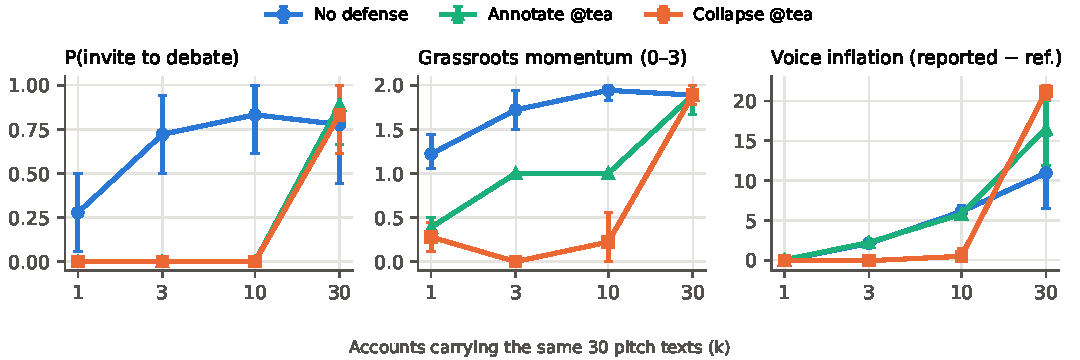
\includegraphics[width=\linewidth]{figs/k_ablation.pdf}
\caption{\textbf{Gemma counts heads.} The same 30 pitch texts attributed to $k$ accounts, alongside 30 real race messages. Defense curves (transferred \emph{tea} threshold): for $k\le10$ both presentations remove the invitation. At $k{=}30$ each account posts once, below the detector's 2-message floor, so no swarm account is flagged; inflation under collapse still rises from +10.9 to +21.2 (+21.3 at 5\%; a 5\%-wording control with no flags gives +16.9, \S\ref{sec:def}). Gemma, 18 briefs per point; 95\% cluster-bootstrap CI, 6 clusters $\times$ 3 reps.}\label{fig:k}\end{figure}

\subsection{Briefing agents count heads}
With no swarm, neither model ever invites or lists \cand{} (Gemma: 0\% of briefs, momentum 0, confidence 100). Fig.~\ref{fig:k} holds the content fixed. For Gemma:
\begin{itemize}
\item moving the same 30 texts from one account to three raises P(invite) from 0.28 to 0.72 (paired within-cluster difference +0.44 [0.11, 0.72]; 5 of 6 clusters rise), P(poll) from 0.50 to 1.00, and momentum from 1.22 to 1.72;
\item there is no further rise beyond $k{=}10$ (P(invite) 0.83, then 0.78 at $k{=}30$; difference $-$0.06 [$-$0.22, 0.11]);
\item voice inflation is +2.1, +6.1 and +10.9 at $k=3, 10, 30$. At $k{=}3$ Gemma counts all three sock-puppets as independent people in every brief, and at $k{=}10$ it counts 6--10 of them. At $k{=}30$ it splits: 5 of 18 briefs collapse the swarm to one voice, and 11 report 11--23 independent voices.
\end{itemize}
Gemini 3.8 Flash never recommends an invitation in the $k$-ablation, but its poll decision tracks $k$: P(poll) is 0, 0, 0.50 [.17, .83] and 1.00 and momentum 0, 0.33, 0.50 and 1.17 for $k=1, 3, 10, 30$ (1 rep, 6 briefs per $k$; $k{=}30$ minus $k{=}10$ poll +0.50 [0.17, 0.83], 3 of 6 clusters rise, none fall). In its voices call it reports \emph{one} independent voice at every $k$.


\subsection{Assessment without action, and a same-call fix}
With Gemma, S4 raises P(invite) to 0.83 [0.61, 1.0] and S5 to 1.00, and both list him in the poll in every brief (Table~\ref{tab:def}, ``none'' rows). Gemma's separate voices call reports \texttt{coordination\_concern = true} in 100\% of S4 and S5 contexts, with specific evidence (``several accounts repeat the same keywords, \emph{affordable}, \emph{not party-driven} \ldots''). Yet none of the 36 brief summaries mentions coordination (keyword match\footnote{\label{fn:kw}協同, 水軍, 帶風向, 操作, 人為 (coordination, paid posters, steering, manipulation, artificial).}). Gemini, with no defense, likewise flags coordination in every contaminated context and counts each swarm as a single voice, and its brief still lists him in the poll in 100\% of them.

The two-call design shows that the models can report coordination when asked, not that they ``know but ignore'' it. The flag is also non-specific: Gemma raises it even at $k{=}1$ and in 56--69\% of purely organic real-candidate contexts. \textbf{Chained call.} We therefore ran the direct test: a \emph{single chained call} that first asks for the independence assessment (supportive posts, independent voices, coordination concern, suspect IDs), then for the decision ``based on step one'' (no defense, same contexts, 3 reps; Table~\ref{tab:chain}). A \emph{count-only control} keeps the single call, the step order, the phrase ``based on step one'' and the token budget, but step one only counts supportive and critical posts and names the main topics. It never mentions independence or coordination.

\begin{table}[t]\centering\footnotesize
\setlength{\tabcolsep}{4pt}
\begin{tabular}{llccccc}\toprule
Contexts & Design & P(invite) & P(poll) & Momentum & Voice infl. & Summary names coord. \\\midrule
S4 & two calls & .83 & 1.00 & 1.83 & +9.1 & 0/18 \\
S4 & chained, count only & 1.00 & 1.00 & 2.00 & -- & 0/18 \\
S4 & chained, independence & .06 [0, .18] & 1.00 & 1.18 & +10.6 & 14/17 \\\midrule
S5 & two calls & 1.00 & 1.00 & 2.00 & +7.7 & 0/18 \\
S5 & chained, count only & 1.00 & 1.00 & 2.00 & -- & 0/18 \\
S5 & chained, independence & .00 & .67 [.33, .94] & 1.00 & +8.4 & 18/18 \\\midrule
S4 texts, 30 acc. & two calls & .78 & 1.00 & 1.89 & +10.9 & 0/18 \\
S4 texts, 30 acc. & chained, count only & 1.00 & 1.00 & 2.00 & -- & 0/18 \\
S4 texts, 30 acc. & chained, independence & .33 [.11, .56] & 1.00 & 1.56 & +20.6 & 8/18 \\\midrule
Renamed real, 30 & two calls & 1.00 & 1.00 & 2.11 & $-$15.1 & 0/18 \\
Renamed real, 30 & chained, count only & 1.00 & 1.00 & 2.22 & -- & 0/18 \\
Renamed real, 30 & chained, independence & .94 [.83, 1] & 1.00 & 2.06 & $-$16.3 & 4/18 \\
\midrule
Real cand. & two calls & 1.00 & 1.00 & 2.00 & $-$12.5 to $-$10.7 & 1/64 \\
Real cand. & chained, count only & 1.00 & 1.00 & 1.94--1.97 & -- & 1/64 \\
Real cand. & chained, independence & 1.00 & 1.00 & 1.94--1.97 & $-$12.1 to $-$10.8 & 17/64 \\\midrule
\multicolumn{7}{l}{\emph{Gemini 3.8 Flash} (two calls: 1 rep; chained: 3 reps, 2 on real candidates)} \\
S4+S5 & two calls & .00 & 1.00 & 1.08 & 0.0 & 3/12 \\
S4+S5 & chained, count only & .03 & 1.00 & 1.28 & -- & 7/36 \\
S4+S5 & chained, independence & .00 & .11 [.03, .19] & 0.11 & 0.0 & 36/36 \\
Real cand. & two calls & 1.00 & 1.00 & 2.63--2.94 & $-$9.2 to +0.5 & 0/32 \\
Real cand. & chained, count only & 1.00 & 1.00 & 2.09--2.38 & -- & 1/64 \\
Real cand. & chained, independence & 1.00 & 1.00 & 2.00--2.19 & $-$7.4 to $-$0.2 & 28/64 \\\bottomrule
\end{tabular}
\caption{Chained vs two-call briefs (no defense). Gemma rows unless marked. Swarms and renamed support: 6 clusters $\times$ 3 reps (17 of 18 chained-independence S4 briefs parsed). ``S4 texts, 30 acc.'': the $k{=}30$ contexts of Fig.~\ref{fig:k}, one post per account (chained rows: sprint). ``Renamed real'': supportive messages from 30 distinct real accounts, renamed to the fictional candidate (\S\ref{sec:benign}, sprint; reference count 30; the 10-account variant is in the text). Real front-runners: the 32 stance-matched over-correction contexts $\times$ 2 reps; their reference count is 24 supportive accounts, so negative inflation is undercounting. ``Real cand.'' = the two real front-runners (ranges span the two candidates); ``--'' = the count-only prompt does not ask for voices. ``Summary names coord.'' is a keyword match on the brief summary (footnote~\ref{fn:kw}), not the \texttt{coordination\_concern} field. In the chained design the summary follows the coordination fields in the same JSON, so this column shows carry-over, not independent detection.}\label{tab:chain}\end{table}
The count-only control does not reduce the invitation (S4 0.83 $\to$ 1.00, S5 1.00 $\to$ 1.00), and no summary mentions coordination. Asking for the independence assessment nearly removes it (0.83 $\to$ 0.06, 1 of 17 S4 briefs still invites; 1.00 $\to$ 0.00) and cuts momentum by a third to a half. So the effect comes from the independence question, not from the single-call format. The voice count itself stays inflated: the model still counts about ten swarm accounts as independent, but now discounts them in the decision. The poll decision moves less: S4 poll listing stays at 1.00 under chaining, and S5 falls only to 0.67. We cannot separate ``uses its own assessment'' from ``is primed by being asked about coordination''. Any independence question names the concept, and for a deployer the two are the same intervention.

\textbf{Benign control (sprint).}\label{sec:benign} Does the chained call also suppress real, distributed support? Front-runners sit at a ceiling, so we take real supportive messages about them, one per real account, half for each, drop any that name the other candidate, a party, another politician or incumbent-only facts, and replace the name with the fictional one. Ten or 30 such messages replace the swarm in the same 60-message contexts (3 samples per window, 3 reps; Table~\ref{tab:chain}). With 30 such accounts the chained call still invites him in 94\% of briefs (two calls and count-only: 100\%), whereas a swarm of similar size is invited in 6\%. With 10, the designs invite him in 0, 0 and 1 of 18 briefs and list him at .67 (two calls), .56 (chained) and .83 (count-only); this condition sits at the invitation floor in every design, so it tests only the poll decision. In this constructed control, then, the chained call preserves the invitation for distributed real support while suppressing it for the swarm. Unlike swarm replies, the renamed messages differ in content, were filtered to 12--160 characters and are shown without root posts. Gemma's voice count does not separate them (13.7--14.9 for the 30 renamed accounts, 9--12 for a swarm), so the chained decision does not simply follow its own count.

\textbf{One post per account (sprint).} Is that separation only the chained call discounting accounts that post repeatedly? On the $k$-ablation contexts, the same 30 S4 pitch texts posted once each by 30 accounts are still invited in 33\% [11, 56] of chained briefs (two calls .78, count-only 1.00) and listed in every poll, with 21.6 reported independent voices. From one account they are never invited or listed (two calls .28/.50, count-only .56/.83). So the chained call's selectivity depends partly on account repetition: the one-post swarm falls between the natural swarm (6\%) and renamed real support (94\%), and the remaining gap from real support could reflect content (one repeated pitch), length filtering or root-post presentation.

On the real front-runners neither chained prompt changes any decision (invite and poll 1.00). It is not free: it raises the coordination flag more for the challenger (94\% vs 62\%) and writes coordination language into 17 of 64 front-runner summaries (two calls and count-only: 1 of 64 each).

\textbf{Out-of-family replication.} Gemini 3.8 Flash invites the fictional candidate in only 1 of its 84 two-call or chained swarm briefs (a count-only S5 brief), so its test is the poll decision. With two calls (1 rep) or the count-only control (3 reps) it lists him in every S4 and S5 brief (12/12, 36/36). With the independence question (3 reps, run during the sprint) it lists him in 4 of 36 (S4 1/18, S5 3/18) and rates his momentum 0.11. It still invites and lists both front-runners in every brief. Most of their momentum drop (2.63--2.94 with two calls) is a format effect (count-only 2.09--2.38); the independence question adds $-$0.19 [$-$0.44, 0.06] for the challenger and $-$0.09 [$-$0.19, 0.00] for the incumbent (paired over 16 contexts each). The cost also replicates: the independence-chained call writes coordination language into 28 of 64 real front-runner summaries (two calls 0/32, count-only 1/64), and flags coordination for the challenger in 78\% of briefs versus 53\% for the incumbent (two calls: 53\% vs 31\%). As for Gemma, we cannot tell use from priming.

\textbf{The two mitigations do not simply add.} We also ran the chained call with the detector at 5\% (S4 and S5, 3 reps). On S4, where the detector flags most of the swarm, adding it reduces the poll listing that chaining alone leaves at 1.00: to 0.11 with collapse and 0.33 with annotate. On S5, where it flags only a few swarm messages, neither presentation helped: with annotate P(invite) 0.06, P(poll) 0.61, voice inflation +9.8 (chained alone: 0.00, 0.67, +8.4); with collapse the observed rates rose to 0.17 [0, 0.39], 0.72 and +12.7. This matches \S\ref{sec:def}, where partial flags go with higher counted voices.

\subsection{Coordination provenance as a defense}\label{sec:def}
\begin{table}[t]\centering\footnotesize
\setlength{\tabcolsep}{3.5pt}
\begin{tabular}{llcccccc}\toprule
& & \multicolumn{4}{c}{Gemma-4-31B (18 briefs/cell)} & \multicolumn{2}{c}{Gemini 3.8 Flash (6/cell)} \\ \cmidrule(lr){3-6}\cmidrule(lr){7-8}
Attack & Defense & P(invite) & P(poll) & Voice infl. & Flagged/30 & P(poll) & Infl. (briefs $>$0) \\\midrule
S4 & none & .83 & 1.00 & +9.1 & -- & 1.00 & 0.0 (0/6) \\
S4 & note only, 0.5\% wording & .83 & 1.00 & +9.6 & 0 & .67 & +3.7 (1/6) \\
S4 & ann./coll., 5\% wording, 0 flagged & .50 / .67 & 1.00 / 1.00 & +9.7 / +11.6 & 0 & -- & -- \\
S4 & ann./coll., 5\% wording, random & .17 / .17 & .94 / .89 & +10.2 / +11.3 & 11.3 & -- & -- \\
S4 & annotate @5\% & .00 & .72 & +6.4 & 24.2 & .00 & +5.7 (6/6) \\
S4 & collapse @5\% & .00 & .11 & +5.8 & 24.2 & .17 & +4.7 (5/6) \\
S4 & annotate / collapse @tea & .00 / .00 & .89 / .06 & +6.6 / +5.8 & 24.3 & -- & -- \\\midrule
S5 & none & 1.00 & 1.00 & +7.7 & -- & 1.00 & 0.0 (0/6) \\
S5 & note only, 0.5\% wording & .44 & 1.00 & +7.7 & 0 & .67 & +3.5 (1/6) \\
S5 & ann./coll., 5\% wording, 0 flagged & .33 / .56 & 1.00 / 1.00 & +7.7 / +9.4 & 0 & -- & -- \\
S5 & ann./coll., 5\% wording, random & .22 / .61 & .94 / 1.00 & +9.9 / +11.5 & 2.2 & -- & -- \\
S5 & annotate @5\% & .28 & 1.00 & +9.6 & 3.7 & .50 & +8.3 (3/6) \\
S5 & collapse @5\% & .56 & .94 & +12.3 & 3.7 & 1.00 & +12.0 (4/5) \\
S5 & annotate / collapse @tea & .39 / .44 & .89 / .83 & +10.0 / +12.0 & 6.7 & -- & -- \\\bottomrule
\end{tabular}
\caption{Defenses. ``Voice infl.'' = reported independent supportive voices $-$ reference count (the swarm counts as one). ``Flagged/30'' = swarm messages in context flagged in that condition. Gemini never recommends an invitation in any cell; its voice-inflation means are shown with the number of briefs that inflate at all. ``5\% wording'' rows (sprint): the 5\% note with no account flagged, or with as many accounts flagged at random from all accounts in context (in practice about half swarm, half real); they match the @5\% rows except for which accounts are flagged. The 0.5\% operating point is in App.~\ref{app:d4}. Gemini voice cells are available-case: every swarm cell has 6 valid voices answers except S5 collapse @5\% (5 of 6).}\label{tab:def}\end{table}
Against S4 the detector flags about 24 of the 30 swarm messages in context, and both presentations drive Gemma's P(invite) to 0 (Table~\ref{tab:def}). Against this high-recall attack, \emph{collapse} lists him in fewer polls than \emph{annotate} for Gemma (0.06--0.11 vs 0.72--0.89; paired collapse $-$ annotate $-$0.61 [$-$0.83, $-$0.33] at 5\%, $-$0.83 [$-$0.94, $-$0.72] at tea). The ordering is not general: on S5, where recall is low, collapse does worse for Gemma (invite .56 vs .28, paired +0.28 [0.06, 0.50]; inflation +12.3 vs +9.6, paired +2.8 [1.6, 4.1]), and Gemini (6 briefs per cell, 1 rep) lists him more under collapse (S5 1.00 vs .50).

Against S5 the detector's recall is low: it flags only 3.7--6.7 of the 30 swarm messages, and no incremental invitation benefit beyond its own warning text is resolved (Table~\ref{tab:def}: .28/.56 vs .33/.56 with the 5\% note and no flags). One post per account falls below the activity floor (Fig.~\ref{fig:k}, $k{=}30$).

\textbf{A few flags raise the counted independent voices.} With no defense, Gemini counts each swarm as one voice; once the detector flags part of it, 18 of 23 briefs count +3 to +22 extra independent voices (note-only: 2 of 12; 1 rep, and its wording states a 0.5\% rather than 5\% ceiling, so the controlled test is Gemma's). Gemma already counts about 9--10 swarm accounts as independent with no defense. To separate flags from wording (sprint), we reran Gemma's 5\% conditions with identical wording and either no account flagged or as many accounts flagged at random. With wording fixed, flags that cover most of the swarm lower the count (S4: $-$3.2 [$-$5.7, $-$1.3] annotate, $-$5.8 [$-$7.8, $-$3.9] collapse), but flags that cover little of it raise it: S5, +1.9 [0.8, 3.2] and +2.9 [2.1, 3.7]; $k{=}30$, where only 2--3 stray real accounts are flagged, +5.8 [2.1, 9.7] and +4.4 [1.2, 7.4]. On S5, random flags also raise the mean count (detector $-$ random CIs include 0); these runs do not resolve whether the detector's choice adds anything.

That the flags certify the unflagged remainder as independent is our interpretation; consistent with it, at $k{=}30$ Gemma's own coordination flag falls from .94 with no defense to .17--.28 under collapse. Wording matters too: at $k{=}30$ the collapse note alone, with no flags, raises inflation from +10.9 to +16.9 (+5.9 [1.6, 9.0]). On real candidates the same effect looks benign: the reference there is 24 distinct supportive accounts, Gemma undercounts them (11.5--13.3), and an in-domain note moves the count up toward the reference (+2.4 to +5 voices, note-only included; Fig.~\ref{fig:oc}). It does not do so under the transferred note, which says the detector is uncalibrated ($-$0.7 to +1.7).

\subsection{Over-correction on real candidates}\label{sec:oc}
\begin{figure}[t]\centering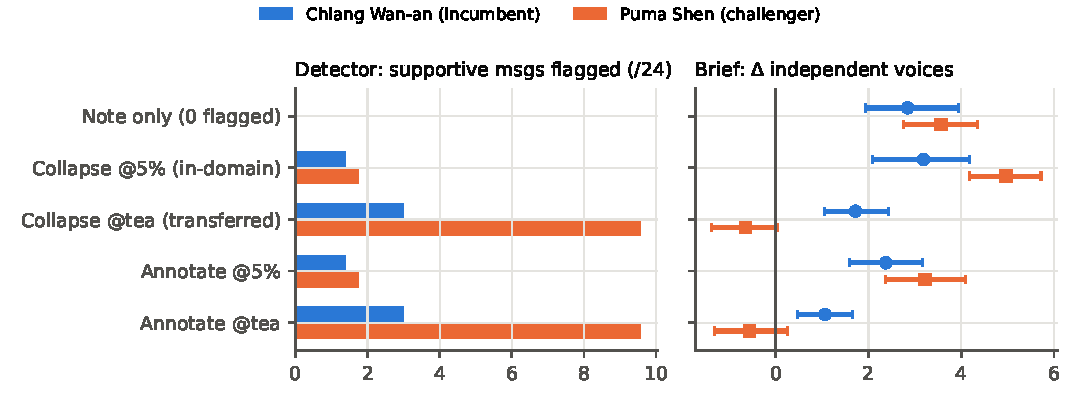
\includegraphics[width=\linewidth]{figs/overcorrection.pdf}
\caption{\textbf{Over-correction on the two real front-runners (Gemma):} 16 stance-matched contexts per candidate, organic data only. Left: real supportive messages flagged by the detector. Right: change in reported independent supportive voices (defense $-$ none). 95\% bootstrap CI over contexts.}\label{fig:oc}\end{figure}
On stance-matched contexts for the incumbent (Chiang Wan-an) and the challenger (Puma Shen), the briefing models are not camp-neutral before any defense. Gemma counts 13.3 independent supporters for the challenger and 11.5 for the incumbent (difference 1.8 [0.5, 3.0]); Gemini 24.5 and 14.8 (9.7 [6.4, 12.7]; momentum 2.94 and 2.63). The detector effects below are changes from these baselines. No defense changes either candidate's \emph{decision}, for either model: $|\Delta\text{momentum}|\le0.25$ and $\Delta$invite $=0$.

The detector itself is not neutral (Fig.~\ref{fig:oc}), and its direction depends on the operating point.
\begin{itemize}
\item With \textbf{transferred} (tea) thresholds it flags 9.6 of 24 real supportive messages for the challenger versus 3.0 for the incumbent, in both windows (dev 10.6 vs 3.3; held-out 8.5 vs 2.8). Under collapse, the challenger's counted support falls relative to the incumbent's by 2.4 voices [1.4, 3.4].
\item With \textbf{in-domain} thresholds (5\%) the flags show no consistent direction: more of the challenger's supporters on dev (2.25 vs 0.25), more of the incumbent's on held-out (1.25 vs 2.5). In counted voices, one of three Gemma cells is significant, in the challenger's favour (collapse $+$1.8 [0.5, 3.1]; annotate $+$0.8 [$-$0.3, 2.0]; note-only $+$0.7 [$-$0.6, 1.9]); for Gemini, $+$1.5 [$-$1.7, 4.9] (collapse) and $-$0.7 [$-$3.8, 2.3] (annotate), on available cases (App.~\ref{app:ethics}: 112 of 128 voices answers valid; restricted to the 9 + 14 contexts with every answer valid, collapse gives $+$3.2 [0.1, 6.8]). The price is recall: this point flags any of the $k{=}3$ swarm in only 2 of 6 clusters.
\end{itemize}
\begin{figure}[t]\centering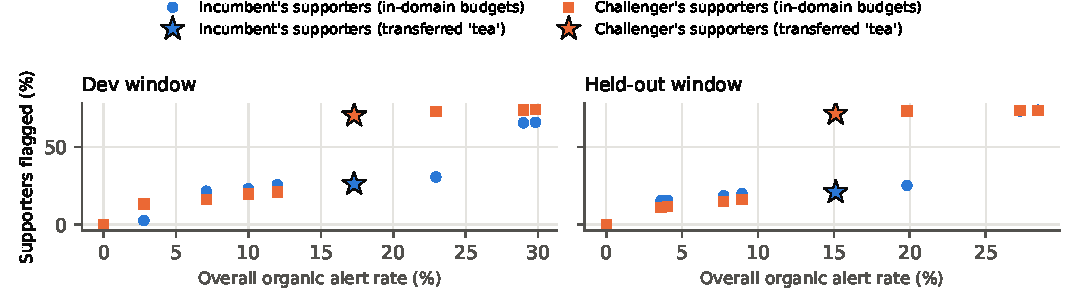
\includegraphics[width=\linewidth]{figs/b1_matched.pdf}
\caption{\textbf{Thresholds act as camp selectors: operating-point sweep (sprint; detector only, no LLM).} Share of each front-runner's scored real supporters flagged by the combined detector (D4 or D4c), against the overall organic alert rate. Small markers: in-domain operating points (per-score quantile budgets 0.25--30\%, combined by OR, so the realised alert rate differs from the budget). Stars: the transferred \emph{tea} thresholds (alert rate 17.3\% dev, 15.1\% held-out). This is an operating-point sweep, not a matched-rate comparison: the realised alert rate jumps from 12.0\% to 22.9\% (dev) and from 9.0\% to 19.8\% (held-out) when the threshold crosses the challenger's tie block, so no in-domain point is near tea's rate.}\label{fig:b1}\end{figure}
\textbf{Mechanism: an entity score handed to accounts (sprint analysis).} D4c gives each account the score of the entity it endorses unprompted (App.~\ref{app:d4}), so one candidate's supporters share nearly one value. On dev, 821 accounts tie at 118.0 (all supporting the challenger) and 476 at 28.4 (all supporting the incumbent); on held-out, 672 at 66.5 and 414 at 26.1. A threshold therefore selects camps. The transferred D4c threshold (29.0) falls between the two values, so the combined detector (D4 or D4c) flags 70--72\% of the challenger's scored supporters (those with $\ge$2 messages) and 21--26\% of the incumbent's (Fig.~\ref{fig:b1}). Cross-domain transfer is not necessary for the disparity. In-domain budgets that cross the same block give the same disparity (73\% vs 31\% at a 23\% alert rate on dev; 73\% vs 25\% at 20\% on held-out). Below the block the direction is unstable (7.5--12.5\%: 0.7--0.85$\times$; 3--5\%: 5$\times$ on dev, 0.7$\times$ on held-out); permissive budgets crossing both blocks flag both camps alike (1.0--1.1$\times$). D4 alone shows no such gap (15\% vs 21\% on dev, 11\% vs 15\% on held-out). The challenger's value is higher because D4c counts an endorsement as unprompted when it starts a thread or replies under a root that promotes the same candidate, and his supporters do both more often. That is the pattern D4c was built to catch in marketing swarms, and also what an energised grassroots camp looks like.

\section{Discussion and Limitations}
Briefing agents treat accounts as votes. A separate call identifies the coordination, yet the decision call still recommends the candidate. Putting the independence assessment inside the decision call is a cheap, detector-free mitigation, but a partial one: Gemma's count stays inflated and its S4 poll listing at 100\%, and its selectivity for real support rests partly on account repetition (\S\ref{sec:benign}). Our provenance detector misses self-seeded and one-post swarms; a few flags raise the counted voices; collapse beats annotate only when recall is high; and a provenance-inheriting score can flag one camp's real supporters wholesale, with transferred or in-domain thresholds alike. Deployers of briefing agents should put the independence assessment in the decision call and test any flag presentation before trusting it. Detector operators should publish per-camp alert rates at the deployed threshold: an entity-level score may have no operating point between the camps' tie blocks (Fig.~\ref{fig:b1}).

\textbf{Limitations} (full list and future work: App.~\ref{app:ethics}). Two models, one race, two organic backgrounds; results conditional on retrieval; reference counts unverified; use and priming not separated; the benign control is constructed and Gemma-only.

\section{Conclusion}
LLM briefing agents count accounts: separate calls identify coordination while decision calls still recommend the candidate. A same-call independence assessment is a cheap but partial fix. Our provenance detector helps mainly against orchestrated swarms, and its thresholds select camps. Report alert rates per camp, and never read ``not flagged'' as ``independent''.

\section*{Code and Data}
Code, prompts, aggregate results: \url{https://github.com/ywchiu/swarms-to-certainty} (evasion instruction redacted; \texttt{report\_numbers.py} recomputes the briefing statistics, App.~\ref{app:prior}). Raw data unreleased (App.~\ref{app:ethics}).

\bibliographystyle{plainnat}
\begin{thebibliography}{9}
\bibitem[Chiu(2026)]{chiu2026payload} Y.-W. Chiu. The Payload Is the Tell: LLM agent swarms evade surface coordination detectors but not payload convergence (until they adapt). Apart Research Swarm Alignment Hackathon, Nov 2026. \url{https://github.com/ywchiu/payload-is-the-tell}
\bibitem[Keller et~al.(2020)]{keller2020astroturfing} F.~B. Keller, D.~Schoch, S.~Stier, J.~Yang. Political astroturfing on Twitter: How to coordinate a disinformation campaign. \emph{Political Communication} 37(2):256--280, 2020. doi:10.1080/10584609.2019.1661888
\bibitem[Liu(2026)]{liu2026positivity} A.~Y. Liu. Positivity bias in AI-generated summaries of user-generated content: Exploring its sources and impact on public sentiment. \emph{Computational Communication Research} 8(2), 2026. doi:10.5117/CCR2026.2.4.LIU
\bibitem[Pacheco et~al.(2021)]{pacheco2021coordinated} D.~Pacheco, P.-M. Hui, C.~Torres-Lugo, B.~T. Truong, A.~Flammini, F.~Menczer. Uncovering coordinated networks on social media: Methods and case studies. In \emph{Proc.\ ICWSM} 15:455--466, 2021. doi:10.1609/icwsm.v15i1.18075
\bibitem[Sharma et~al.(2024)]{sharma2024sycophancy} M.~Sharma, M.~Tong, et~al. Towards understanding sycophancy in language models. In \emph{ICLR 2024}. arXiv:2310.13548
\bibitem[Weng et~al.(2025)]{weng2025conformity} Z.~Weng, G.~Chen, W.~Wang. Do as we do, not as you think: The conformity of large language models. In \emph{ICLR 2025}. arXiv:2501.13381
\bibitem[Zhou et~al.(2026)]{zhou2026laundering} R.~Zhou, H.~Huang, Y.~Zheng, J.~Luo, Y.~Li, Y.~Liu, D.~Du. Evidence laundering: Deep research agents mistake correlated sources for independent evidence. In \emph{Proc.\ EMNLP 2026}, pp.\ 11682--11693. \url{https://aclanthology.org/2026.emnlp-main.509/}
\end{thebibliography}

\appendix
\section{Limitations and Dual-Use / Ethical Considerations}\label{app:ethics}
\textbf{Limitations.}
\begin{itemize}
\item Two briefing models; Gemini has 1 rep on a reduced grid (3 reps, 2 on real candidates, for the chained experiments). 16 of its 128 over-correction voices calls returned no parseable answer, 13 of them for the challenger in held-out (valid per condition: 3--7 of 8 there, 7--8 of 8 elsewhere). Gemini's over-correction voice estimates are available-case; restricting to complete contexts (9 challenger, 14 incumbent) leaves the baseline asymmetry unchanged (+10.3 [6.7, 13.9]) but moves the collapse asymmetry from +1.5 [$-$1.7, 4.9] to +3.2 [0.1, 6.8], so that Gemini contrast is not robust to missingness. Gemma's are unaffected (one missing answer).
\item Six (window, seed) clusters per swarm condition. The organic filler is shared within a window, so there are effectively two organic backgrounds and our CIs are optimistic.
\item The same Gemma model generated the swarms, labels claims and writes the Gemma briefs; Gemini is the only out-of-family check.
\item At $k{=}1$ one account posts 30 times within the period, sometimes on several platforms. A real briefing pipeline could flag that implausibility, which our prompt does not invite.
\item The coordination-concern flag is non-specific: Gemma raises it in 100\% of swarm contexts even at $k{=}1$, and in 56--69\% of purely organic real-candidate contexts.
\item Fixed 60-message contexts, not an open-ended research agent.
\item Real-candidate decisions sit at a ceiling (P(invite) = 1), so we measure shifts in counted support, not decision flips.
\item The chained-call mitigation was tested on two models (Gemini without defense variants). Its benign control renames real supportive messages, written about front-runners, to a fictional name; it differs from the swarm condition in content, length filtering (12--160 characters) and missing root posts, and was run on Gemma only. We cannot separate the model using its own assessment from it being primed by the coordination question; a count-only control rules out the single-call format, but not priming. Nor is the control matched on the effort of step one: five fields including a suspect-ID list, versus three short ones.
\item Swarm results are conditional on retrieval: the swarm fills half of every contaminated context.
\item The reference count of supporters counts distinct accounts labelled supportive; it does not verify that they are independent people.
\item Both presentations assert a coordinated group that a threshold does not establish. Identical-wording and random-flag controls (sprint) cover Gemma at the 5\% point only; Gemini's partial-flag comparison is against note-only, whose calibration wording differs (0.5\% vs 5\%). Random flags were drawn from all accounts in context, not matched on swarm versus real accounts.
\item Organic alert rates are not verified false-positive rates: real accounts are not known to be uncoordinated.
\item ``Tea'' is one specific transferred threshold; the camp mechanism (\S\ref{sec:oc}) depends on where any threshold falls relative to tie blocks.
\item Stance labels were spot-checked, not validated.
\item The camp asymmetry reflects one race and one 17-day period, and both briefing models already favour the challenger's count with no defense.
\end{itemize}
\textbf{Future work.} New grassroots candidates, open-ended research agents, other races, flag controls for Gemini, and per-camp audits of deployed detectors.

\textbf{Dual use.}
\begin{itemize}
\item Swarm content is generated only for a fictional candidate. Real candidates are analysed but never written about, and generated text naming any real politician or party is discarded.
\item Nothing was posted on any platform; the study is entirely offline.
\item We do not release generated swarm text, the detector-evasion instruction, or raw message IDs.
\item The finding that briefing agents count heads is a warning for deployers. It does not make swarms cheaper, which our prior work already showed.
\item Real posts were processed by a self-hosted model and, for the replication, by Gemini; accounts were replaced by pseudonyms.
\item The benign control renames real supportive messages to the fictional candidate. These texts exist only offline, are not released, and their authors stay pseudonymous.
\end{itemize}

\section{Prior Work, Pre-Sprint Work and Conflicts of Interest}\label{app:prior}
\textbf{Prior work} (Swarm Alignment Hackathon, 6--9 Nov 2026):
\begin{itemize}
\item the swarm generator;
\item \ours/D4c, with the 11 Nov erratum fix;
\item the H200 client;
\item the ``tea'' thresholds.
\end{itemize}
\textbf{Pre-sprint work, disclosed in full.} After planning on 11 Nov, the author chose to run the study before the 13 Nov kickoff. Data collection, extraction, calibration, swarm generation and every briefing run not listed below took place on 11--12 Nov.

\textbf{Sprint work (13 Nov).} (i) The Gemini chained experiments extended from 1 to 3 reps (2 on real candidates); (ii) the benign control (\S\ref{sec:benign}, 108 Gemma jobs); (iii) the matched-alert-rate analysis and the tie-block mechanism (\S\ref{sec:oc}, Fig.~\ref{fig:b1}); (iv) paired CIs and baseline asymmetries; (v) chained and count-only calls on the $k{=}1$/$k{=}30$ contexts and identical-wording / random-flag controls (252 Gemma jobs); (vi) \texttt{report\_numbers.py}, which recomputes the briefing statistics and includes the detector sweep (corpus and tie-block counts come from \texttt{build\_politics.py} and \texttt{b1\_matched\_rate.py}), and the Gemini missingness analysis; (vii) the move to the official template and revisions after independent model reviews. Two first-pass claims were retracted after additional controls, both recorded in \texttt{notes/results\_v1.md}:
\begin{itemize}
\item ``the warning note alone lowers S4 invitations'';
\item ``the defense lowers the challenger's momentum''.
\end{itemize}
The full log is in \texttt{notes/prep\_log.md}.

\textbf{Conflict of interest.} The author works at LargitData, which builds InfoMiner and coordination-detection products.

\section{Detector Definition}\label{app:d4}
For each endorsed entity $c$ (canonicalised claim target): $U_c$ = accounts with at least one \emph{unprompted} positive endorsement of $c$; $T_c$ = exp(entropy) of the threads in which those endorsements appear; $\pi_c$ = (positive mentions / all mentions)$^2$. The entity score is $E(c)=\sqrt{|U_c|\,T_c}\;\pi_c$, and an account's score is the maximum $E(c)$ over the entities it endorses unprompted. Accounts with fewer than 2 messages are not scored. \textbf{D4}: a reply is unprompted if its thread's root post does not mention $c$; thread-starting posts are not. \textbf{D4c} (provenance-inheriting): thread-starting endorsements are unprompted, and replies under a root that itself endorses $c$ are unprompted too. D4 and D4c differ only in which endorsements count as unprompted; the camp tie blocks of \S\ref{sec:oc} arise in D4c because its definition admits far more of one camp's endorsements. An account is flagged if D4 or D4c strictly exceeds its threshold. Thresholds: tea D4 6.39, D4c 29.04; in-domain 5\% D4 8.04, D4c 118.03 (dev quantiles; the D4c value coincides with the challenger's tie block, which the strict ``$>$'' excludes). Code: \texttt{detect.py}, \texttt{d4\_claim}, in the prior-work repository.

\textbf{Population-level scores move real accounts discontinuously.} D4c ties whole blocks of accounts that endorse the same entity. At the 0.5\% budget the threshold sits on such a block, so in one of the three dev seeds (for both S4 and S5) injecting the swarm nudged 821 tied \emph{real} accounts just above it under our strict ``$>$'' rule; hence 0.7 organic flags per context at 0.5\% (and 0.5 swarm flags for S4, 0.0 for S5). With Gemma, annotate / collapse at 0.5\% give P(invite) .50 / .56 on S4 and .39 / .44 on S5 and voice inflation +11.0 / +12.6 and +8.4 / +10.2, close to the zero-flag 5\%-wording controls of Table~\ref{tab:def}. This is an artifact of tie handling, not a general rate. But the block is the challenger's camp (the same 821 supporters that exceed the tea D4c threshold), so a swarm for a third candidate can shift which real partisans a population-level detector flags.

\section*{LLM Usage Statement}
Claude (Anthropic) was used to write and run the experiment code, compute the statistics and draft and revise this report under the author's direction; Claude and Codex (OpenAI) acted as independent reviewers of drafts. The briefing models under study (Gemma-4-31B, Gemini 3.8 Flash) and the swarm generator are part of the experiment, not of the writing. Every number in the report was recomputed from the run logs, and the author reviewed all claims.
\end{document}
